\section{Data Description and Sources}\label{sec:data}

Our final dataset has \nAdults adults and 26 columns (Table~\ref{tab:dictionary}). It is built from four public US government sources: one person-level survey stacked over five years, and three regional tables joined on region and year.

\subsection*{Dataset composition at a glance}\label{sec:composition}

Every rate, odds ratio and correlation in this report is computed on a stated subset of the adults below, so we first show what the data are made of (Tables~\ref{tab:comp-years}--\ref{tab:comp-groups}; source: \file{reports/tables/dataset_composition.csv}, produced by \file{supplementary_analysis.py}). Each survey year contributes between 27,594 and 31,925 adults and between 112 and 145 cases, so no single year dominates (Table~\ref{tab:comp-years}). The 26 columns of the clean file are of nine kinds (Table~\ref{tab:comp-columns}): one identifier, one survey weight and the target, which are never features; two numeric columns, four ordinal, three nominal and seven binary survey variables; four engineered columns; and three regional columns joined on region and year. The model-ready file keeps \nFeatures of the \nCandidates candidate features (Section~\ref{sec:selection}), grouped in Table~\ref{tab:comp-groups}. Finally, the stratified 80/20 split keeps the same \sampleRate\% case rate in the \nTrain training rows and the \nTest test rows (Table~\ref{tab:comp-years}, lower part). Unless stated otherwise, descriptive numbers use all \nAdults adults with the variable known, and anything that ranks or fits features uses the training rows only.

\begin{table}[htbp]
\centering\small
\caption{Adults and lung-cancer cases per survey year, and in the train / test split (unweighted).}\label{tab:comp-years}
\begin{tabular}{lrrr}
\toprule
 & Adults & Cases & Rate (sample) \\
\midrule
2019 & 31,925 & 112 & 0.35\% \\
2020 & 31,513 & 131 & 0.42\% \\
2021 & 29,430 & 115 & 0.39\% \\
2022 & 27,594 & 116 & 0.42\% \\
2023 & 29,466 & 145 & 0.49\% \\
\textbf{All years} & \textbf{149,928} & \textbf{619} & \textbf{0.41\%} \\
\midrule
Training rows & 119,942 & 495 & 0.41\% \\
Test rows & 29,986 & 124 & 0.41\% \\
\bottomrule
\end{tabular}

\end{table}

\begin{table}[htbp]
\centering\small
\caption{The 26 columns of the clean dataset by type.}\label{tab:comp-columns}
\begin{tabularx}{\textwidth}{l r >{\raggedright\arraybackslash}X}
\toprule
Type & Columns & Which \\
\midrule
Identifier & 1 & person\_id \\
Survey weight & 1 & survey\_weight \\
Target & 1 & lung\_cancer \\
Numeric & 2 & age, year \\
Ordinal & 4 & education, income\_group, general\_health, bmi\_category \\
Nominal & 3 & race\_ethnicity, region, smoking\_status \\
Binary & 7 & sex, ever\_ecigarette, copd, asthma, hypertension, heart\_disease, diabetes \\
Engineered & 4 & age\_group, ever\_smoker, screening\_age\_smoker, comorbidity\_count \\
Regional (joined) & 3 & pm25\_mean, smoking\_rate, lung\_cancer\_incidence \\
\midrule
\textbf{Total} & \textbf{26} &  \\
\bottomrule
\end{tabularx}

\end{table}

\begin{table}[htbp]
\centering\small
\caption{The \nFeatures final model features by group (full list in Appendix~\ref{app:features}).}\label{tab:comp-groups}
\begin{tabularx}{\textwidth}{l >{\raggedright\arraybackslash}X r}
\toprule
Group & Features & Count \\
\midrule
Demographic & age (scaled); sex: Female (reference: Male); race/ethnicity: AIAN, AIAN and other, Asian, Black, Hispanic, Other or multiple (reference: White) & 8 \\
Socio-economic & education: Bachelor, Graduate, Less than high school, Some college, Unknown (reference: High school / GED); income vs poverty line: Below poverty, Low, Middle (reference: High) & 8 \\
Smoking and nicotine & screening\_age\_smoker; screening\_age\_smoker\_unknown; ever\_ecigarette; ever\_ecigarette\_unknown; smoking status: Current, Former (reference: Never) & 6 \\
Health & copd; asthma; hypertension; heart\_disease; diabetes; general health: Fair, Good, Poor, Very good (reference: Excellent); BMI category: Obese, Overweight, Underweight, Unknown (reference: Healthy) & 13 \\
Regional context & pm25\_mean (scaled); smoking\_rate (scaled); lung\_cancer\_incidence (scaled) & 3 \\
\midrule
\textbf{Total} &  & \textbf{38} \\
\bottomrule
\end{tabularx}

\end{table}

\subsection{Sources and provenance}\label{sec:sources}

\begin{table}[htbp]
\centering\small
\caption{Data sources, publisher, granularity and raw size.}\label{tab:sources}
\begin{tabularx}{\textwidth}{@{}r >{\raggedright\arraybackslash}X >{\raggedright\arraybackslash}p{2.9cm} >{\raggedright\arraybackslash}p{2.6cm} >{\raggedright\arraybackslash}p{2.7cm} >{\raggedright\arraybackslash}p{2.4cm}@{}}
\toprule
\# & Source & Publisher & One raw row is & Raw size & Used for \\
\midrule
1 & National Health Interview Survey, Sample Adult files 2019--2023~\cite{nhis} & CDC -- National Center for Health Statistics & one adult in one survey year & \nRawRows adults (27,651--31,997 per year) & individual features and the target \\
2 & EPA AirData, annual concentration by monitor, 2019--2023~\cite{epa} & US Environmental Protection Agency & one monitor $\times$ pollutant $\times$ year & 75,534--107,019 rows per year & regional PM2.5 pollution \\
3 & BRFSS prevalence data, current smokers, 2019--2023~\cite{brfss} & CDC Behavioral Risk Factor Surveillance System & one state $\times$ year $\times$ answer & 1,644 rows & regional adult smoking rate \\
4 & US Cancer Statistics, incidence by area~\cite{uscs} & CDC and National Cancer Institute & one area $\times$ year $\times$ sex $\times$ race $\times$ site & 23,796 lung-cancer rows & regional lung-cancer incidence \\
\bottomrule
\end{tabularx}
\end{table}

All four sources are public-domain US government data (Table~\ref{tab:sources}), so we can commit them to the repository. The raw files were downloaded on 24--25 October 2026 with \file{scripts/download_data.py}, which fetches them again from the official URLs in the References if they are missing. They sit unchanged in \file{data/raw/}, and we only ever change data through code, never by hand -- the ``never overwrite the original'' rule of the course (Chapter~2). The three regional files were reduced to the rows we need at download time so that every file stays under GitHub's 100~MB limit; the reduction is done in code and is fully reproducible.

\subsection{Granularity and target definition}\label{sec:granularity}

One row is one surveyed adult (18+) in one survey year. NHIS interviews one randomly selected adult per household, so the household number plus the survey year (\file{person_id}) identifies a row. The regional sources are coarser -- a monitor, or a state -- and the public NHIS files only reveal the person's US Census region (Northeast, Midwest, South, West). We therefore aggregated every regional measure to region $\times$ year, so each regional column takes only $4 \times 5 = 20$ distinct values and describes the person's environment, not the person.

\textbf{The target.} \file{lung_cancer} is 1 if the person reports that a doctor ever told them they had lung cancer. NHIS does not ask this in a single question, so we derive it from two: ``ever told you had cancer?'' (\file{CANEV_A}) and, only for people who said yes, ``what kind?'' (\file{LUNGCAN_A}). The target is 0 for people who never had cancer and for people who had a different cancer.

\subsection{Data dictionary}\label{sec:dictionary}

\begin{table}[htbp]
\centering\small
\caption{Data dictionary of the final clean dataset (26 columns); the type follows Table~\ref{tab:comp-columns}. Full version: \texttt{data/clean/data\_dictionary.csv}.}\label{tab:dictionary}
\begin{tabularx}{\textwidth}{>{\raggedright\arraybackslash}p{3.8cm} >{\raggedright\arraybackslash}X l >{\raggedright\arraybackslash}p{3.4cm}}
\toprule
Column & Meaning & Type & Built from \\
\midrule
person\_id & Unique ID: survey year + NHIS household number & identifier & NHIS HHX + SRVY\_YR \\
year & Survey year (2019-2023) & numeric & SRVY\_YR \\
survey\_weight & NHIS sampling weight (use for population estimates) & weight & WTFA\_A \\
age & Age in years (85 = 85 or older) & numeric & AGEP\_A \\
sex & Male / Female & binary & SEX\_A \\
race\_ethnicity & Hispanic origin and race & nominal & HISPALLP\_A \\
region & US region & nominal & REGION \\
education & Highest education level (grouped) & ordinal & EDUC\_A (EDUCP\_A from 2021) \\
income\_group & Family income vs poverty line: below (<1), low (1-2), middle (2-4), high (4+) & ordinal & RATCAT\_A \\
general\_health & Self-rated general health & ordinal & PHSTAT\_A \\
bmi\_category & Body mass index category & ordinal & BMICAT\_A \\
smoking\_status & Cigarette smoking: Current / Former / Never & nominal & SMKCIGST\_A \\
ever\_ecigarette & Ever used an e-cigarette (1 = yes) & binary & ECIGEV\_A \\
copd & Ever told COPD, emphysema or chronic bronchitis (1 = yes) & binary & COPDEV\_A \\
asthma & Ever had asthma (1 = yes) & binary & ASEV\_A \\
hypertension & Ever told high blood pressure (1 = yes) & binary & HYPEV\_A \\
heart\_disease & Ever told coronary heart disease (1 = yes) & binary & CHDEV\_A \\
diabetes & Ever told diabetes (1 = yes) & binary & DIBEV\_A \\
age\_group & NEW: age band & engineered & from age \\
ever\_smoker & NEW: current or former smoker (1 = yes) & engineered & from smoking\_status \\
screening\_age\_smoker & NEW: age 50-80 and ever smoked (proxy of screening eligibility) & engineered & from age + smoking \\
comorbidity\_count & NEW: number of the 5 conditions above & engineered & from copd...diabetes \\
pm25\_mean & JOINED: average fine-particle air pollution (PM2.5, µg/m³) in the person's region that year & regional & EPA AirData, by region + year \\
smoking\_rate & JOINED: \% of adults who currently smoke in the person's region that year & regional & CDC BRFSS, by region + year \\
lung\_cancer\_incidence & JOINED: new lung cancer cases per 100,000 people in the person's region that year & regional & CDC US Cancer Statistics, by region + year \\
lung\_cancer & TARGET: ever told they had lung cancer (1 = yes) & target & CANEV\_A + LUNGCAN\_A \\
\bottomrule
\end{tabularx}

\end{table}

\subsection{Target distribution}\label{sec:target}

\begin{figure}[htbp]
\centering
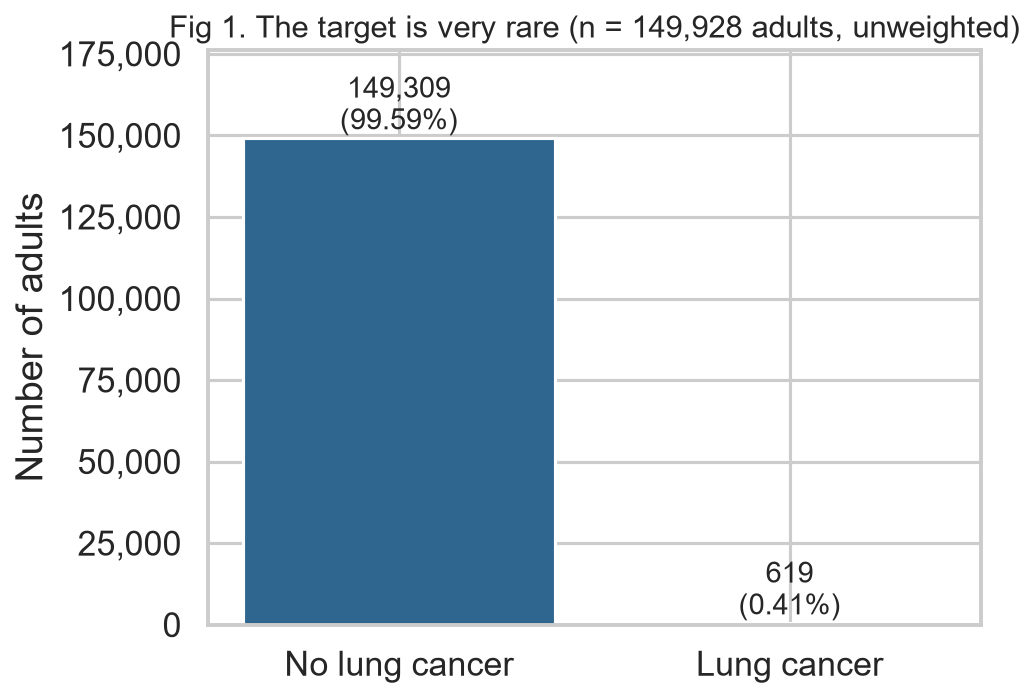
\includegraphics[width=0.55\textwidth]{fig01_class_balance}
\caption{Class balance of the target. Only \nCases of \nAdults adults (\sampleRate\%) report a lung-cancer diagnosis; the population rate after NHIS survey weighting is 0.31\%.}\label{fig:balance}
\end{figure}

The imbalance is extreme (Fig.~\ref{fig:balance}): a model that always answers ``no'' would be 99.59\% accurate while finding no one. This single number drove our choice of effect sizes (odds ratios rather than accuracy-like measures), of a stratified train/test split, and of the metrics planned for the modelling phase.

\subsection{Who is in the data: a detailed profile of the study population}\label{sec:profile}

Before testing anything, we describe exactly who the \nAdults adults are and where the \nCases cases sit. Tables~\ref{tab:prof-demo}--\ref{tab:prof-conditions} give, for every category of every variable, the number of adults, their share of the sample and of the US adult population (survey-weighted), the number of adults with and without a lung-cancer history, the lung-cancer rate in the sample and in the population, and the mean age of the group. ``Unknown'' rows are people who did not give a usable answer; we keep them so that every block adds up to \nAdults adults and \nCases cases (shares therefore differ slightly from Fig.~\ref{fig:categorical}, which uses known answers only). All numbers come from \file{reports/tables/population_profile.csv}, produced by \file{scripts/supplementary_analysis.py}.

Two reading rules apply throughout. First, the sample rate is what we observe among the people interviewed, while the weighted rate estimates the rate among all US adults: NHIS interviews some groups more than others (for example, 31.1\% of the adults with a known age are 65 or older, against 21.9\% of the population), and the survey weights correct for this. Second, raw counts of cases depend on group size: 507 of the \nCases cases are White adults simply because White adults are 67.5\% of the sample, so groups are compared through their rates, never through their counts.

\subsubsection{Demographics: sex, age and race/ethnicity}\label{sec:demo}

\begin{table}[htbp]
\centering\footnotesize
\caption{Demographic profile of the \nAdults adults: adults, share of the sample and of the US adult population (weighted, wtd), adults with and without a lung-cancer history, lung-cancer rate and mean age, by sex, age group and race/ethnicity. AIAN = American Indian or Alaska Native.}\label{tab:prof-demo}
\begin{tabular*}{\textwidth}{@{\extracolsep{\fill}}lrrrrrrrr}
\toprule
Group & Adults & \makecell[b]{\% of\\{}sample} & \makecell[b]{\% of US\\{}adults (wtd)} & \makecell[b]{Lung\\{}cancer} & \makecell[b]{No lung\\{}cancer} & \makecell[b]{Rate\\{}(sample)} & \makecell[b]{Rate\\{}(wtd)} & \makecell[b]{Mean\\{}age} \\
\midrule
\textbf{Sex} &  &  &  &  &  &  &  &  \\
\quad Female & 81,360 & 54.3 & 51.5 & 354 & 81,006 & 0.44\% & 0.32\% & 53.6 \\
\quad Male & 68,552 & 45.7 & 48.5 & 265 & 68,287 & 0.39\% & 0.30\% & 51.9 \\
\quad Unknown & 16 & 0.0 & 0.0 & 0 & 16 & 0.00\% & 0.00\% & 37.6 \\
\midrule
\textbf{Age group (years)} &  &  &  &  &  &  &  &  \\
\quad 18--44 & 54,481 & 36.3 & 45.8 & 13 & 54,468 & 0.02\% & 0.02\% & 32.4 \\
\quad 45--54 & 21,574 & 14.4 & 15.7 & 21 & 21,553 & 0.10\% & 0.08\% & 49.6 \\
\quad 55--64 & 27,020 & 18.0 & 16.5 & 113 & 26,907 & 0.42\% & 0.45\% & 59.7 \\
\quad 65--74 & 26,445 & 17.6 & 13.0 & 222 & 26,223 & 0.84\% & 0.81\% & 69.3 \\
\quad 75+ & 20,055 & 13.4 & 8.9 & 249 & 19,806 & 1.24\% & 1.25\% & 80.5 \\
\quad Unknown & 353 & 0.2 & 0.2 & 1 & 352 & 0.28\% & 0.11\% & -- \\
\midrule
\textbf{Race / ethnicity} &  &  &  &  &  &  &  &  \\
\quad White & 101,181 & 67.5 & 62.5 & 507 & 100,674 & 0.50\% & 0.39\% & 55.3 \\
\quad Hispanic & 20,411 & 13.6 & 17.0 & 27 & 20,384 & 0.13\% & 0.10\% & 45.0 \\
\quad Black & 16,138 & 10.8 & 11.8 & 55 & 16,083 & 0.34\% & 0.22\% & 51.3 \\
\quad Asian & 8,453 & 5.6 & 6.0 & 16 & 8,437 & 0.19\% & 0.22\% & 46.9 \\
\quad AIAN & 962 & 0.6 & 0.7 & 8 & 954 & 0.83\% & 0.60\% & 50.5 \\
\quad AIAN and other & 1,114 & 0.7 & 0.7 & 5 & 1,109 & 0.45\% & 0.43\% & 52.2 \\
\quad Other or multiple & 1,669 & 1.1 & 1.3 & 1 & 1,668 & 0.06\% & 0.02\% & 41.2 \\
\bottomrule
\end{tabular*}

\end{table}

\begin{itemize}
  \item \textbf{Sex.} The sample has 81,360 women (54.3\%) and 68,552 men (45.7\%); after weighting the split is 51.5\% / 48.5\%. More cases are women (354, against 265 men), but women are also more numerous and slightly older (mean age 53.6 vs 51.9 years), and the weighted rates are almost equal (0.32\% vs 0.30\%). Section~\ref{sec:sociodemo} confirms that sex is not associated with lung cancer.
  \item \textbf{Age.} Adults aged 18--44 are the largest group (36.3\% of the sample, 45.8\% of the population) but include only 13 cases (0.02\%). From there the rate climbs steadily: 0.10\% at 45--54, 0.42\% at 55--64, 0.84\% at 65--74 and 1.24\% at 75+. The 46,500 adults aged 65 or older (31.1\% of those with a known age) hold 471 of the \nCases cases (76.1\%; 76.2\% of the 618 cases with a known age, as in Table~\ref{tab:cases}).
  \item \textbf{Race and ethnicity.} NHIS records Hispanic origin and race in one variable; it is the only measure of cultural background in our variable set. The sample has 101,181 White adults (507 with and 100,674 without a lung-cancer history), 20,411 Hispanic adults (27 with, 20,384 without), 16,138 Black adults (55 with, 16,083 without), 8,453 Asian adults (16 with, 8,437 without), and three small groups -- AIAN (American Indian or Alaska Native, 962 adults, 8 cases), AIAN and another group (1,114 adults, 5 cases) and other or multiple races (1,669 adults, 1 case). The weighted rate is highest among White adults (0.39\%) and lowest among Hispanic adults (0.10\%). The three small groups total only 14 cases, so their rates are unstable and they are merged for testing (\S\ref{sec:sociodemo}).
\end{itemize}

\textbf{Why the groups differ.} Table~\ref{tab:group-profile} looks inside each sex and race/ethnicity group. White adults are the oldest group (mean age 55.3, 36.5\% aged 65+) and the most likely, after the AIAN groups, to have ever smoked (42.7\%); Hispanic adults are among the youngest (mean 45.0, 15.5\% aged 65+) and smoke much less (25.0\% ever-smokers). Asian adults have the lowest smoking prevalence (18.3\%). Age and smoking -- the two strongest risk factors in this project -- therefore explain a large part of the raw differences between race/ethnicity groups, which is why we do not interpret those differences as an effect of race itself. Men smoke more than women (43.4\% vs 32.9\% ever-smokers), yet women are older on average and report COPD slightly more often (6.2\% vs 5.0\%), which is consistent with the near-equal rates by sex.

\begin{table}[htbp]
\centering\footnotesize
\caption{Inside each sex and race/ethnicity group: age, sex, smoking and COPD, which explain much of the difference in lung-cancer rates (percentages among adults with a known answer; rate weighted). Source: \texttt{group\_profile.csv}.}\label{tab:group-profile}
\begin{tabular*}{\textwidth}{@{\extracolsep{\fill}}lrrrrrrrrr}
\toprule
Group & Adults & Cases & \makecell[b]{Mean\\{}age} & \makecell[b]{Median\\{}age} & \makecell[b]{\% aged\\{}65+} & \makecell[b]{\%\\{}women} & \makecell[b]{\% ever\\{}smoked} & \makecell[b]{\%\\{}COPD} & \makecell[b]{Rate\\{}(wtd)} \\
\midrule
\textbf{Sex} &  &  &  &  &  &  &  &  &  \\
\quad Female & 81,360 & 354 & 53.6 & 55 & 32.9 & -- & 32.9 & 6.2 & 0.32\% \\
\quad Male & 68,552 & 265 & 51.9 & 53 & 29.0 & -- & 43.4 & 5.0 & 0.30\% \\
\midrule
\textbf{Race / ethnicity} &  &  &  &  &  &  &  &  &  \\
\quad White & 101,181 & 507 & 55.3 & 58 & 36.5 & 53.5 & 42.7 & 6.7 & 0.39\% \\
\quad Hispanic & 20,411 & 27 & 45.0 & 43 & 15.5 & 54.3 & 25.0 & 2.4 & 0.10\% \\
\quad Black & 16,138 & 55 & 51.3 & 52 & 26.2 & 59.0 & 30.9 & 5.2 & 0.22\% \\
\quad Asian & 8,453 & 16 & 46.9 & 44 & 18.5 & 54.2 & 18.3 & 1.0 & 0.22\% \\
\quad AIAN & 962 & 8 & 50.5 & 51 & 23.8 & 57.1 & 50.4 & 10.5 & 0.60\% \\
\quad AIAN and other & 1,114 & 5 & 52.2 & 53.5 & 28.6 & 57.5 & 50.6 & 11.6 & 0.43\% \\
\quad Other or multiple & 1,669 & 1 & 41.2 & 38 & 11.7 & 53.9 & 32.5 & 2.4 & 0.02\% \\
\bottomrule
\end{tabular*}

\end{table}

\subsubsection{Socio-economic position, region and survey year}\label{sec:socio}

\begin{table}[htbp]
\centering\footnotesize
\caption{Socio-economic, geographic and yearly profile (same columns as Table~\ref{tab:prof-demo}). Income is family income divided by the poverty line.}\label{tab:prof-socio}
\begin{tabular*}{\textwidth}{@{\extracolsep{\fill}}lrrrrrrrr}
\toprule
Group & Adults & \makecell[b]{\% of\\{}sample} & \makecell[b]{\% of US\\{}adults (wtd)} & \makecell[b]{Lung\\{}cancer} & \makecell[b]{No lung\\{}cancer} & \makecell[b]{Rate\\{}(sample)} & \makecell[b]{Rate\\{}(wtd)} & \makecell[b]{Mean\\{}age} \\
\midrule
\textbf{Education} &  &  &  &  &  &  &  &  \\
\quad Less than high school & 12,809 & 8.5 & 10.9 & 86 & 12,723 & 0.67\% & 0.49\% & 56.8 \\
\quad High school / GED & 37,368 & 24.9 & 27.5 & 219 & 37,149 & 0.59\% & 0.40\% & 53.7 \\
\quad Some college & 42,452 & 28.3 & 29.2 & 195 & 42,257 & 0.46\% & 0.32\% & 52.4 \\
\quad Bachelor & 34,364 & 22.9 & 19.8 & 64 & 34,300 & 0.19\% & 0.15\% & 50.3 \\
\quad Graduate & 22,175 & 14.8 & 11.9 & 48 & 22,127 & 0.22\% & 0.16\% & 53.5 \\
\quad Unknown & 760 & 0.5 & 0.7 & 7 & 753 & 0.92\% & 0.59\% & 54.5 \\
\midrule
\textbf{Family income vs poverty line} &  &  &  &  &  &  &  &  \\
\quad Below poverty ($<$1) & 15,119 & 10.1 & 10.2 & 95 & 15,024 & 0.63\% & 0.46\% & 50.5 \\
\quad Low (1--2) & 26,307 & 17.5 & 18.0 & 164 & 26,143 & 0.62\% & 0.43\% & 54.2 \\
\quad Middle (2--4) & 44,165 & 29.5 & 30.1 & 187 & 43,978 & 0.42\% & 0.32\% & 53.2 \\
\quad High (4+) & 64,337 & 42.9 & 41.7 & 173 & 64,164 & 0.27\% & 0.21\% & 52.5 \\
\midrule
\textbf{Census region} &  &  &  &  &  &  &  &  \\
\quad Northeast & 24,963 & 16.6 & 17.6 & 117 & 24,846 & 0.47\% & 0.37\% & 53.8 \\
\quad Midwest & 33,049 & 22.0 & 20.8 & 174 & 32,875 & 0.53\% & 0.42\% & 53.2 \\
\quad South & 54,341 & 36.2 & 38.0 & 229 & 54,112 & 0.42\% & 0.29\% & 52.9 \\
\quad West & 37,575 & 25.1 & 23.6 & 99 & 37,476 & 0.26\% & 0.20\% & 51.7 \\
\midrule
\textbf{Survey year} &  &  &  &  &  &  &  &  \\
\quad 2019 & 31,925 & 21.3 & 19.7 & 112 & 31,813 & 0.35\% & 0.28\% & 52.0 \\
\quad 2020 & 31,513 & 21.0 & 19.9 & 131 & 31,382 & 0.42\% & 0.31\% & 53.5 \\
\quad 2021 & 29,430 & 19.6 & 19.9 & 115 & 29,315 & 0.39\% & 0.28\% & 52.5 \\
\quad 2022 & 27,594 & 18.4 & 20.1 & 116 & 27,478 & 0.42\% & 0.34\% & 52.9 \\
\quad 2023 & 29,466 & 19.7 & 20.3 & 145 & 29,321 & 0.49\% & 0.34\% & 53.2 \\
\bottomrule
\end{tabular*}

\end{table}

\begin{itemize}
  \item \textbf{Education.} The largest groups are ``some college'' (42,452 adults, 28.3\%) and high school / GED (37,368, 24.9\%; Table~\ref{tab:prof-socio}). The rate falls from 0.67\% (sample) among adults without a high-school diploma to 0.19\% among bachelor's graduates; weighted, from 0.49\% to 0.15\%.
  \item \textbf{Income.} 42.9\% of adults have a family income at least four times the poverty line and 10.1\% live below it. The rate halves from below-poverty (0.46\% weighted) to high income (0.21\%).
  \item \textbf{Region.} The South is the largest region (54,341 adults, 36.2\%), followed by the West (25.1\%), the Midwest (22.0\%) and the Northeast (16.6\%). The weighted rate is highest in the Midwest (0.42\%) and lowest in the West (0.20\%); the matching sample rates are 0.53\% and 0.26\%. The West is also the youngest region (mean age 51.7).
  \item \textbf{Survey year.} Each year contributes 27,594--31,925 adults and 112--145 cases. The rate drifts upward from 0.35\% in 2019 to 0.49\% in 2023 (weighted, 0.28\% to 0.34\%), but the difference between years is not statistically significant ($\chi^2(4) = 7.9$, $p = 0.096$; \file{rate_by_year.csv}). This matters because 2019 was the first year of the redesigned NHIS questionnaire and 2020 collection was disrupted by COVID-19 (largely telephone interviews); because the years do not differ significantly, pooling them is reasonable, and we keep year in the data so the modelling phase can check it again.
\end{itemize}

\subsubsection{Smoking, body weight, self-rated health and chronic conditions}\label{sec:smokingprofile}

\begin{table}[htbp]
\centering\footnotesize
\caption{Smoking, e-cigarette use, body weight and self-rated health (same columns as Table~\ref{tab:prof-demo}).}\label{tab:prof-smoking}
\begin{tabular*}{\textwidth}{@{\extracolsep{\fill}}lrrrrrrrr}
\toprule
Group & Adults & \makecell[b]{\% of\\{}sample} & \makecell[b]{\% of US\\{}adults (wtd)} & \makecell[b]{Lung\\{}cancer} & \makecell[b]{No lung\\{}cancer} & \makecell[b]{Rate\\{}(sample)} & \makecell[b]{Rate\\{}(wtd)} & \makecell[b]{Mean\\{}age} \\
\midrule
\textbf{Cigarette smoking} &  &  &  &  &  &  &  &  \\
\quad Never & 90,937 & 60.7 & 63.5 & 107 & 90,830 & 0.12\% & 0.08\% & 50.3 \\
\quad Former & 37,452 & 25.0 & 22.0 & 367 & 37,085 & 0.98\% & 0.81\% & 59.7 \\
\quad Current & 17,586 & 11.7 & 11.7 & 127 & 17,459 & 0.72\% & 0.60\% & 51.1 \\
\quad Unknown & 3,953 & 2.6 & 2.8 & 18 & 3,935 & 0.46\% & 0.32\% & 52.9 \\
\midrule
\textbf{Ever used an e-cigarette} &  &  &  &  &  &  &  &  \\
\quad No & 122,606 & 81.8 & 79.4 & 497 & 122,109 & 0.41\% & 0.31\% & 55.1 \\
\quad Yes & 23,470 & 15.7 & 17.8 & 105 & 23,365 & 0.45\% & 0.29\% & 41.0 \\
\quad Unknown & 3,852 & 2.6 & 2.8 & 17 & 3,835 & 0.44\% & 0.32\% & 52.7 \\
\midrule
\textbf{BMI category} &  &  &  &  &  &  &  &  \\
\quad Underweight & 2,324 & 1.6 & 1.6 & 33 & 2,291 & 1.42\% & 1.14\% & 51.7 \\
\quad Healthy & 46,153 & 30.8 & 30.7 & 221 & 45,932 & 0.48\% & 0.35\% & 51.6 \\
\quad Overweight & 50,466 & 33.7 & 33.2 & 187 & 50,279 & 0.37\% & 0.29\% & 54.2 \\
\quad Obese & 47,471 & 31.7 & 32.2 & 165 & 47,306 & 0.35\% & 0.24\% & 52.4 \\
\quad Unknown & 3,514 & 2.3 & 2.3 & 13 & 3,501 & 0.37\% & 0.28\% & 54.6 \\
\midrule
\textbf{Self-rated general health} &  &  &  &  &  &  &  &  \\
\quad Excellent & 32,824 & 21.9 & 23.4 & 18 & 32,806 & 0.05\% & 0.03\% & 46.5 \\
\quad Very good & 51,131 & 34.1 & 33.9 & 73 & 51,058 & 0.14\% & 0.10\% & 51.1 \\
\quad Good & 42,973 & 28.7 & 28.3 & 173 & 42,800 & 0.40\% & 0.28\% & 55.4 \\
\quad Fair & 17,483 & 11.7 & 11.1 & 206 & 17,277 & 1.18\% & 0.96\% & 59.8 \\
\quad Poor & 5,457 & 3.6 & 3.3 & 149 & 5,308 & 2.73\% & 2.47\% & 63.4 \\
\quad Unknown & 60 & 0.0 & 0.0 & 0 & 60 & 0.00\% & 0.00\% & 61.5 \\
\bottomrule
\end{tabular*}

\end{table}

\begin{table}[htbp]
\centering\footnotesize
\caption{Chronic conditions (ever told by a doctor) and the number of the five conditions (same columns as Table~\ref{tab:prof-demo}).}\label{tab:prof-conditions}
\begin{tabular*}{\textwidth}{@{\extracolsep{\fill}}lrrrrrrrr}
\toprule
Group & Adults & \makecell[b]{\% of\\{}sample} & \makecell[b]{\% of US\\{}adults (wtd)} & \makecell[b]{Lung\\{}cancer} & \makecell[b]{No lung\\{}cancer} & \makecell[b]{Rate\\{}(sample)} & \makecell[b]{Rate\\{}(wtd)} & \makecell[b]{Mean\\{}age} \\
\midrule
\textbf{COPD} &  &  &  &  &  &  &  &  \\
\quad No & 141,386 & 94.3 & 95.3 & 330 & 141,056 & 0.23\% & 0.17\% & 52.0 \\
\quad Yes & 8,440 & 5.6 & 4.6 & 288 & 8,152 & 3.41\% & 3.13\% & 65.4 \\
\quad Unknown & 102 & 0.1 & 0.1 & 1 & 101 & 0.98\% & 0.32\% & 64.8 \\
\midrule
\textbf{Heart disease} &  &  &  &  &  &  &  &  \\
\quad No & 140,524 & 93.7 & 95.0 & 475 & 140,049 & 0.34\% & 0.25\% & 51.6 \\
\quad Yes & 9,073 & 6.1 & 4.8 & 139 & 8,934 & 1.53\% & 1.52\% & 70.7 \\
\quad Unknown & 331 & 0.2 & 0.2 & 5 & 326 & 1.51\% & 1.34\% & 69.9 \\
\midrule
\textbf{Hypertension} &  &  &  &  &  &  &  &  \\
\quad No & 94,990 & 63.4 & 68.2 & 215 & 94,775 & 0.23\% & 0.16\% & 46.7 \\
\quad Yes & 54,776 & 36.5 & 31.7 & 404 & 54,372 & 0.74\% & 0.63\% & 63.3 \\
\quad Unknown & 162 & 0.1 & 0.1 & 0 & 162 & 0.00\% & 0.00\% & 58.7 \\
\midrule
\textbf{Diabetes} &  &  &  &  &  &  &  &  \\
\quad No & 133,796 & 89.2 & 90.4 & 488 & 133,308 & 0.36\% & 0.26\% & 51.4 \\
\quad Yes & 16,064 & 10.7 & 9.5 & 131 & 15,933 & 0.82\% & 0.74\% & 64.5 \\
\quad Unknown & 68 & 0.0 & 0.0 & 0 & 68 & 0.00\% & 0.00\% & 59.7 \\
\midrule
\textbf{Asthma} &  &  &  &  &  &  &  &  \\
\quad No & 129,025 & 86.1 & 85.8 & 502 & 128,523 & 0.39\% & 0.29\% & 53.2 \\
\quad Yes & 20,839 & 13.9 & 14.2 & 116 & 20,723 & 0.56\% & 0.41\% & 50.2 \\
\quad Unknown & 64 & 0.0 & 0.0 & 1 & 63 & 1.56\% & 2.55\% & 57.4 \\
\midrule
\textbf{Number of the 5 conditions} &  &  &  &  &  &  &  &  \\
\quad 0 & 76,217 & 50.8 & 55.2 & 87 & 76,130 & 0.11\% & 0.08\% & 45.9 \\
\quad 1 & 47,541 & 31.7 & 29.9 & 203 & 47,338 & 0.43\% & 0.33\% & 57.0 \\
\quad 2 & 18,719 & 12.5 & 10.8 & 166 & 18,553 & 0.89\% & 0.74\% & 64.2 \\
\quad 3 & 5,808 & 3.9 & 3.2 & 118 & 5,690 & 2.03\% & 2.05\% & 67.1 \\
\quad 4 & 1,426 & 1.0 & 0.8 & 36 & 1,390 & 2.52\% & 2.24\% & 68.0 \\
\quad 5 & 217 & 0.1 & 0.1 & 9 & 208 & 4.15\% & 3.79\% & 66.7 \\
\bottomrule
\end{tabular*}

\end{table}

\begin{itemize}
  \item \textbf{Smoking.} 90,937 adults have never smoked (60.7\% of all adults, 62.3\% of those who answered), 37,452 are former and 17,586 current smokers; 3,953 did not answer. Former smokers have the highest rate (0.98\% sample, 0.81\% weighted) and are much older (mean age \formerSmokerAge, against 51.1 for current and 50.3 for never-smokers), a first hint of the reverse causation discussed in \S\ref{sec:rq1}.
  \item \textbf{E-cigarettes.} 23,470 adults (15.7\%) have ever used one. They are much younger (mean age 41.0 vs 55.1), which is why their crude rate (0.29\% weighted) is close to that of non-users (0.31\%).
  \item \textbf{Body weight and self-rated health.} Underweight adults are only 1.6\% of the sample but have the highest rate (1.42\%, 33 cases). Self-rated health shows the steepest gradient in the whole dataset: 0.05\% for ``excellent'' up to 2.73\% for ``poor'' (sample rates), with 149 cases among the 5,457 adults in poor health.
  \item \textbf{Chronic conditions.} 8,440 adults (5.6\%) report COPD, and 288 of them have a lung-cancer history -- 46.5\% of all cases, at a rate of 3.41\%, fifteen times the 0.23\% of adults without COPD. About half of adults (50.8\%) have none of the five conditions; the rate then rises with every additional condition, from 0.11\% with none to 4.15\% with all five.
\end{itemize}

\subsubsection{Adults with and without a lung-cancer history, side by side}\label{sec:sidebyside}

Table~\ref{tab:cases} summarises the same information from the other direction: what the \nCases cases look like compared with the 149,309 other adults. Cases are about 18.5 years older on average (71.2 vs 52.7), are more than twice as likely to have ever smoked (82.2\% vs 37.5\%), are eight times as likely to report COPD (46.6\% vs 5.5\%) and almost four times as likely to rate their health as fair or poor (57.4\% vs 15.1\%). They are more often White (81.9\% vs 67.4\%) and less often Hispanic (4.4\% vs 13.7\%) -- a difference that the age and smoking profiles of Table~\ref{tab:group-profile} largely explain -- and the share of women is similar (57.2\% vs 54.3\%).

\begin{table}[htbp]
\centering\small
\caption{Characteristics of adults with and without a lung-cancer history (unweighted; percentages among adults with a known answer). Source: \texttt{cases\_vs\_noncases.csv}.}\label{tab:cases}
\begin{tabular}{lrr}
\toprule
Characteristic & Lung cancer & No lung cancer \\
\midrule
Adults & 619 & 149,309 \\
Age, mean (years) & 71.2 & 52.7 \\
Age, standard deviation (years) & 10.2 & 18.3 \\
Age, median (years) & 72.0 & 54.0 \\
Age, interquartile range (years) & 65--79 & 37--68 \\
Aged 65 or older & 76.2\% & 30.9\% \\
Female & 57.2\% & 54.3\% \\
Race/ethnicity -- White & 81.9\% & 67.4\% \\
Race/ethnicity -- Hispanic & 4.4\% & 13.7\% \\
Race/ethnicity -- Black & 8.9\% & 10.8\% \\
Race/ethnicity -- Asian & 2.6\% & 5.7\% \\
Race/ethnicity -- AIAN / other / multiple & 2.3\% & 2.5\% \\
Ever smoked (former or current) & 82.2\% & 37.5\% \\
Current smoker & 21.1\% & 12.0\% \\
Ever used an e-cigarette & 17.4\% & 16.1\% \\
COPD & 46.6\% & 5.5\% \\
Heart disease & 22.6\% & 6.0\% \\
Hypertension & 65.3\% & 36.5\% \\
Diabetes & 21.2\% & 10.7\% \\
Asthma & 18.8\% & 13.9\% \\
Comorbidity count, mean & 1.7 & 0.7 \\
Fair or poor self-rated health & 57.4\% & 15.1\% \\
Underweight & 5.4\% & 1.6\% \\
Obese & 27.2\% & 32.4\% \\
Less than high school & 14.1\% & 8.6\% \\
Bachelor or graduate degree & 18.3\% & 38.0\% \\
Family income below the poverty line & 15.3\% & 10.1\% \\
Region -- Northeast & 18.9\% & 16.6\% \\
Region -- Midwest & 28.1\% & 22.0\% \\
Region -- South & 37.0\% & 36.2\% \\
Region -- West & 16.0\% & 25.1\% \\
\bottomrule
\end{tabular}

\end{table}

\subsection{Initial data-quality issues and limitations}\label{sec:quality}

\begin{itemize}
  \item \textbf{Severe imbalance:} \nCases cases out of \nAdults adults (\sampleRate\%).
  \item \textbf{Hidden missing values:} NHIS stores ``refused / not ascertained / don't know'' as numbers (7, 8, 9 or 97, 98, 99) that look like real values; 4,424 such codes sat in just four key columns.
  \item \textbf{A renamed column:} education is \file{EDUC_A} in 2019--2020 but \file{EDUCP_A} from 2021 (same codes), and code 11 (doctorate) exists only in 2019--2020.
  \item \textbf{Self-reported, lifetime answers:} someone diagnosed years ago may have quit smoking or lost weight since, so current habits can be a result of the cancer (reverse causation).
  \item \textbf{No smoking dose:} NHIS has no pack-years or quit dates, so we can only approximate the official screening group.
  \item \textbf{Survey design:} NHIS is not a simple random sample. It over-samples some groups -- the sample is older than the population (31.1\% aged 65+ vs 21.9\% after weighting) -- so raw rates (\sampleRate\%) differ from population rates (0.31\%).
  \item \textbf{Year comparability:} the 2019 questionnaire redesign and the 2020 pandemic disruption could affect comparability between years; the year-to-year differences in the case rate are not significant ($p = 0.096$).
  \item \textbf{Coarse regional data:} each regional variable has only 20 distinct values (4 regions $\times$ 5 years), so it is ecological context, not personal exposure.
  \item \textbf{Possible repeats across years:} people cannot be linked between survey years, so a few adults may appear in two different years.
\end{itemize}

\subsection{The dataset we rejected}\label{sec:rejected}

We started the project with a 22,457-row file (\file{lung_cancer_combined_22457.csv}, no documented origin) that has the same columns as the well-known 309-person Kaggle lung-cancer survey~\cite{kaggle}. Before using it we audited it the way we would review an unknown dependency, and it failed review (Table~\ref{tab:audit}). The decisive evidence is the row order and the lineage; duplicates and label conflicts alone would be weak evidence, because a file with about fifteen low-cardinality columns produces repeated answer patterns naturally.

\begin{table}[htbp]
\centering\small
\caption{Integrity audit of the supplied file (all numbers recomputed from the file), strongest evidence first.}\label{tab:audit}
\begin{tabularx}{\textwidth}{@{}>{\raggedright\arraybackslash}p{2.6cm} >{\raggedright\arraybackslash}X >{\raggedright\arraybackslash}p{4.6cm}@{}}
\toprule
Check & Finding & Why it matters \\
\midrule
Row order & the first 1,455 rows are all negative; the first positive label appears at row 1,456 & row position (and \texttt{patient\_id}) predicts the label -- a leakage path \\
Lineage & only 1,438 rows (6.4\%) match a row of the public 309-person survey (252 of its patterns, one repeated 59 times; labels agree in 99.4\% of matches); the other 21,019 rows match no public source & most of the file has no traceable origin \\
Signal after deduplication & no feature is associated with the label (all Cram\'er's $V < 0.02$) & the apparent signal came from the duplicates and the ordered block \\
Exact duplicates & 2,573 rows repeat another row exactly & the same answers counted many times inflate every statistic \\
Label conflicts & 133 identical answer patterns carry both labels (315 rows) & the label is not a clean function of the answers \\
\bottomrule
\end{tabularx}
\end{table}

This pattern is statistically consistent with resampling or programmatic generation; it is not proof that the data are synthetic. We replaced the file with NHIS and kept it in \file{data/raw/other/} so the decision stays auditable. The lineage numbers were recomputed against an identical public copy of the Kaggle survey~\cite{kaggle}.
